%%%%%%%%%%%%%%%%%%%%%%%%%%%%%%%%%%%%%%%%%%%%%%%%%%%%%%%%%%%%%%%%%%%%%%%%%%
%%%%%                         CHAPITRE 2                            %%%%%%
%%%%%%%%%%%%%%%%%%%%%%%%%%%%%%%%%%%%%%%%%%%%%%%%%%%%%%%%%%%%%%%%%%%%%%%%%%

\lhead[\fancyplain{}{\leftmark}]%Pour les pages paires \bfseries
      {\fancyplain{}{}} %Pour les pages impaires
\chead[\fancyplain{}{}]%
      {\fancyplain{}{}}
\rhead[\fancyplain{}{}]%Pour les pages paires 
      {\fancyplain{}{\rightmark}}%Pour les pages impaires \bfseries
\lfoot[\fancyplain{}{}]%
      {\fancyplain{}{}}
\cfoot[\fancyplain{}{\thepage}]%\bfseries
      {\fancyplain{}{\thepage}} %\bfseries
\rfoot[\fancyplain{}{}]%
     {\fancyplain{}{\scriptsize}}


%%%%%%%%%%%%%%%%%%%%%%%%%%%%%%%%%%%%%%%%%%%%%%%%%%%%%%%%%%%%%%%%%%%%%%%%%%
%%%%%                      Start part here                          %%%%%%
%%%%%%%%%%%%%%%%%%%%%%%%%%%%%%%%%%%%%%%%%%%%%%%%%%%%%%%%%%%%%%%%%%%%%%%%%%

\chapter{Theoretical framework}
\label{ch:2}

%==============================================================================	Résumé du chapitre

\begin{center}
\rule{0.7\linewidth}{.5pt}
\begin{minipage}{0.7\linewidth}
\smallskip

\textit{Obtaining coherent 3D kinematics from a network of calibrated video cameras involves understanding a certain theoretical framework. First, keypoints must be recognized in images. This is mostly achieved with machine learning models. Then, all the 2D features detected for each camera need to be reconstructed in the 3D space. Finally, these coordinates must be constrained to an anatomically consistent model, in order to obtain coherent 3D joint kinematics.}

%\smallskip
\end{minipage}
\smallskip
\rule{0.7\linewidth}{.5pt}
\end{center}

\minitoc
\newpage

\section{Introduction}

Sports movements don’t generally only lie in the sagittal plane, and they often cause body part occlusions. Moreover, although the need is not as strong as for clinical applications, it is important for results to be as biomechanically coherent as possible. Hence, one of the most promising prospects for sports movement analysis consists in addressing the problem with several video sources, and then constraining 3D coordinates to a kinematic model.  Such research is at the intersection of machine learning for 2D pose estimation, computer vision for 3D reconstruction from a network of calibrated videos, and biomechanics for constraining 3D point coordinates to an anatomically consistent model, in order to obtain reliable kinematics. 


\section{2D pose detection}

\subsection{Why machine learning?}

As a first step, achieving motion analysis from a network of cameras involves detecting features in images. These features can be whole human beings, joint centers, body landmarks, sports gear such as tennis balls, climbing holds, or much more. 

Two broad approaches can be implemented: the first one consists in using dedicated algorithms for each task. The gist of it is to understand the task well enough to build an appropriate solution: this is a knowledge-driven approach. Among other techniques, corner and contour detection, color thresholding, affine transformation, template matching, watershed segmentation, can be used. For example, if one wants to differentiate two boxers wearing respectively a blue and a red shirt, they can filter them by color. If one needs to identify on which portion of a speed climbing wall an athlete is, they can match the template of each holds on the whole image. OpenCV \cite{Bradski2000} provides convenient tools for this purpose, in C++ and Python languages. This approach is often fast, but also quite complicated to implement, and neither flexible nor robust. If there is other red or blue patches in the boxing scene, if the boxer wears green or if the light is poor, this will not work anymore. Likewise for holds, if the sun casts a large shadow which changes its apparent shape, or if holds are seen from a different perspective.

% Ajouter triangulation de tracked keypoints (sans ML), plutôt que de kpt/obj détection ? SOURCES? CITER KINOVEA, EXPLORER UN PEU VISP 

The second approach takes advantage of machine learning algorithms, which constitute an entirely different paradigm. The idea is to show the machine enough examples for it to "understand" by itself its underlying attributes, so that it manages to detect and label automatically new images: this is a data-driven approach. It can be used for both aforementioned tasks, in a much more flexible way: if one wants the system to recognize boxing gloves or holds in challenging conditions, they simply have to include such examples while training the model. The machine learning approach is also suitable for other tasks, such as whole-image classification (e.g., determining whether this is a boxing or a BMX scene), object detection (e.g., localization of a bike and of a person with a bounding box), background extraction \cite{Bouwmans2019}, semantic and instance segmentation (e.g., extracting the shape of the bike and of the person) \cite{Minaee2021}, or keypoint detection (e.g., localization of human joint centers and keypoints on a bike \cite{Chen2020}) (Figure~\ref{fig_classif_detec}). By 2015, data-driven methods definitely took over knowledge-driven ones in vision analysis problems, and by extension in sports motion analysis from videos (Figure~\ref{fig_exp}).

\clearpage
\begin{figure}[!ht]
	\centering
	\def\svgwidth{1\columnwidth}
	\fontsize{10pt}{10pt}\selectfont
	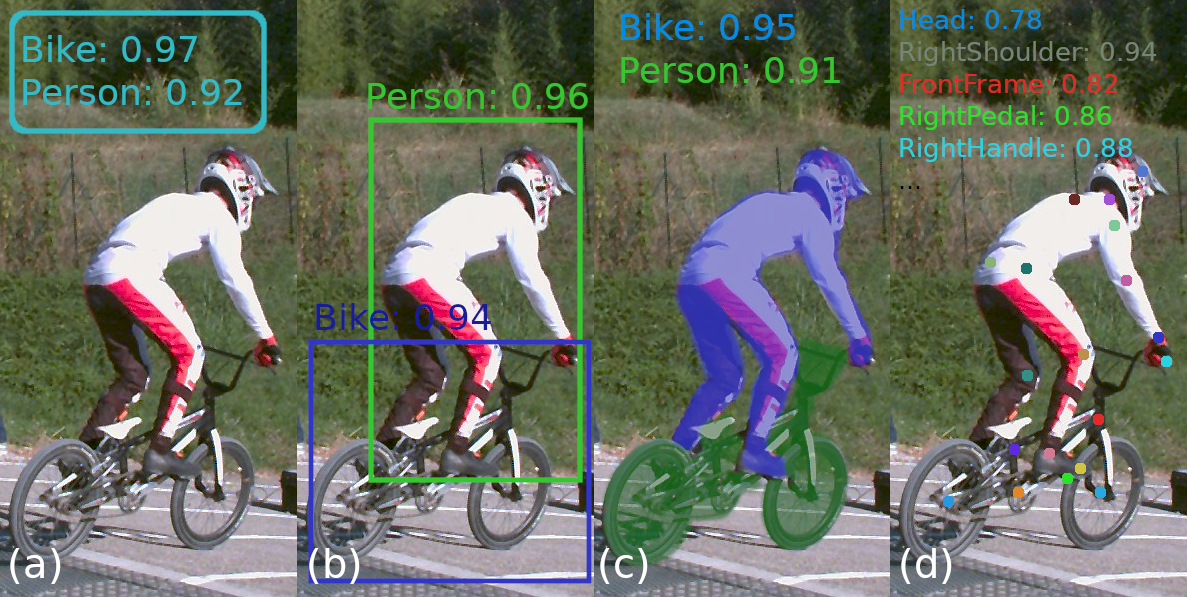
\includegraphics[width=\linewidth]{"../Chap2/Figures/Fig_classif_detec.png"}
	\caption{Mock examples of different types of image analysis. (a) Whole image classification, (b) Object detection and localization, (c) Instance segmentation and shape extraction, (d) Keypoint detection.}
	\label{fig_classif_detec}
\end{figure}

\subsection{Machine learning timeline and principles}

Machine learning is a subset of artificial intelligence (AI.) As such, one can trace its origin back to the discovery of the natural neuron at the end of the 19th century, by Nobel Prize Ramón y Cajal \cite{Lopez2006}, followed half a century later by the first model of an artificial neuron \cite{Mcculloch1943}. A natural neuron is a simple learning unit, which collects the nervous influx sent by other neurons to its dendrites, and sends an action potential when the total influx weighted and summed in the soma overcomes a threshold value. This potential is then transmitted through the axon to the next neuron as a new influx. Similarly, an artificial neuron receives output vectors from previous neurons, weighs and sums them with a summation function, and transfers the resulting output vector to the next neurons if it reaches a certain threshold determined by an activation function (Figure~\ref{fig_neuron}a-b). 

The perceptron, invented in 1956 \cite{Rosenblatt1958}, represents the first practical application of an artificial neuron. It acts as a binary classifier which predicts class 1 if the neuron is fired, and class 0 otherwise. It automatically adjusts its weights by learning from previously labeled example data (see Algorithm~\ref{alg:perceptron} and Figure~\ref{fig_neuron}b). It could be used, for example, to predict whether an athlete is going to be "good" or not, given his force-velocity results on an ergometer test (see step-by-step \hyperlink{example1}{Example 1} and Figure~\ref{fig_perceptron}), and given enough example data. Needing previously labeled data makes it is a supervised classifier – we will not discuss unsupervised methods here. Of course, this example is oversimplified. Being good or not as a sport is a complex and multifactorial outcome, and two variables can't sum it up. However, the perceptron can take more than two variables as inputs (for example, force, velocity, and endurance), and it can also be generalized to multiclass classification with more than two outputs (for example, to differentiate between strong, explosive, and resistant type of athletes.)

Nevertheless, it often takes a lot of iterations over good quality training data for the perceptron to converge. Moreover, it does converge if and only if the data are linearly separable, i.e., if they can be separated with a straight line \cite{Novikoff1963} (see Figure~\ref{fig_linearly_sep}). Some fundamental problems such as the XOR gate can't be solved with a basic single layer Artificial Neural Network (ANN) \cite{Minsky1969}. This constituted one of the early setbacks for AI. Then, the high computational cost of these approaches, combined with the complexity of common-sense problems, hampered the trust in learning methods. Indeed, vision and language problems require enormous amounts of data, and can't be solved with a simple dictionary (for example, "the spirit is willing but the flesh is weak" becomes "the vodka is good but the meat is rotten" when translated back and forth from English to Russian.) Overinflated promises and expectations, followed by disappointment in academia and industries, led to cuts in funding, and eventually loss of skills in the 1970s: this is referred to as the first AI winter.

The AI field survived by focusing on specific problems, called expert systems. In the early 1980s, a new rise was triggered by massive funding such as the Japanese Fifth Generation Computer project, aiming to build a supercomputer that could solve any problem. Shortly after, multi-layer neural networks were made possible with the (re)discovery of backpropagation \cite{Rumelhart1986}, or more rigorously of weight adjustment thanks to the backpropagation of error gradient, from the last layer to the first one. As it is not the central subject of this thesis, the algorithm and early references will not be detailed here, but the interested reader can refer to \cite{Goodfellow2016}. This allowed for solving non-linearly separable problems, and for tackling real world issues (Figure~\ref{fig_neuron}c.). \cite{Cybenko1989} proved that one single intermediate layer is enough to solve any given classification problem, granted that this layer contains enough neurons (although sometimes too many to make it possible in practice.) On the other hand, kernel tricks were also rediscovered \cite{Aizerman1964,Hofmann2008}, and made non-neural networks such as support vector machines (SVMs) \cite{Boser1992} able to treat non-linearly separable data with much less training data, more optimally, and on a clearer mathematical ground (Figure~\ref{fig_linearly_sep}). However, again, unrealistic expectations were confronted with unplanned technical difficulties both on expert systems and on general intelligence projects. This led to a second AI winter in the 1990s. 


\begin{figure}[hbtp]
	\centering
	\def\svgwidth{1\columnwidth}
	\fontsize{10pt}{10pt}\selectfont
	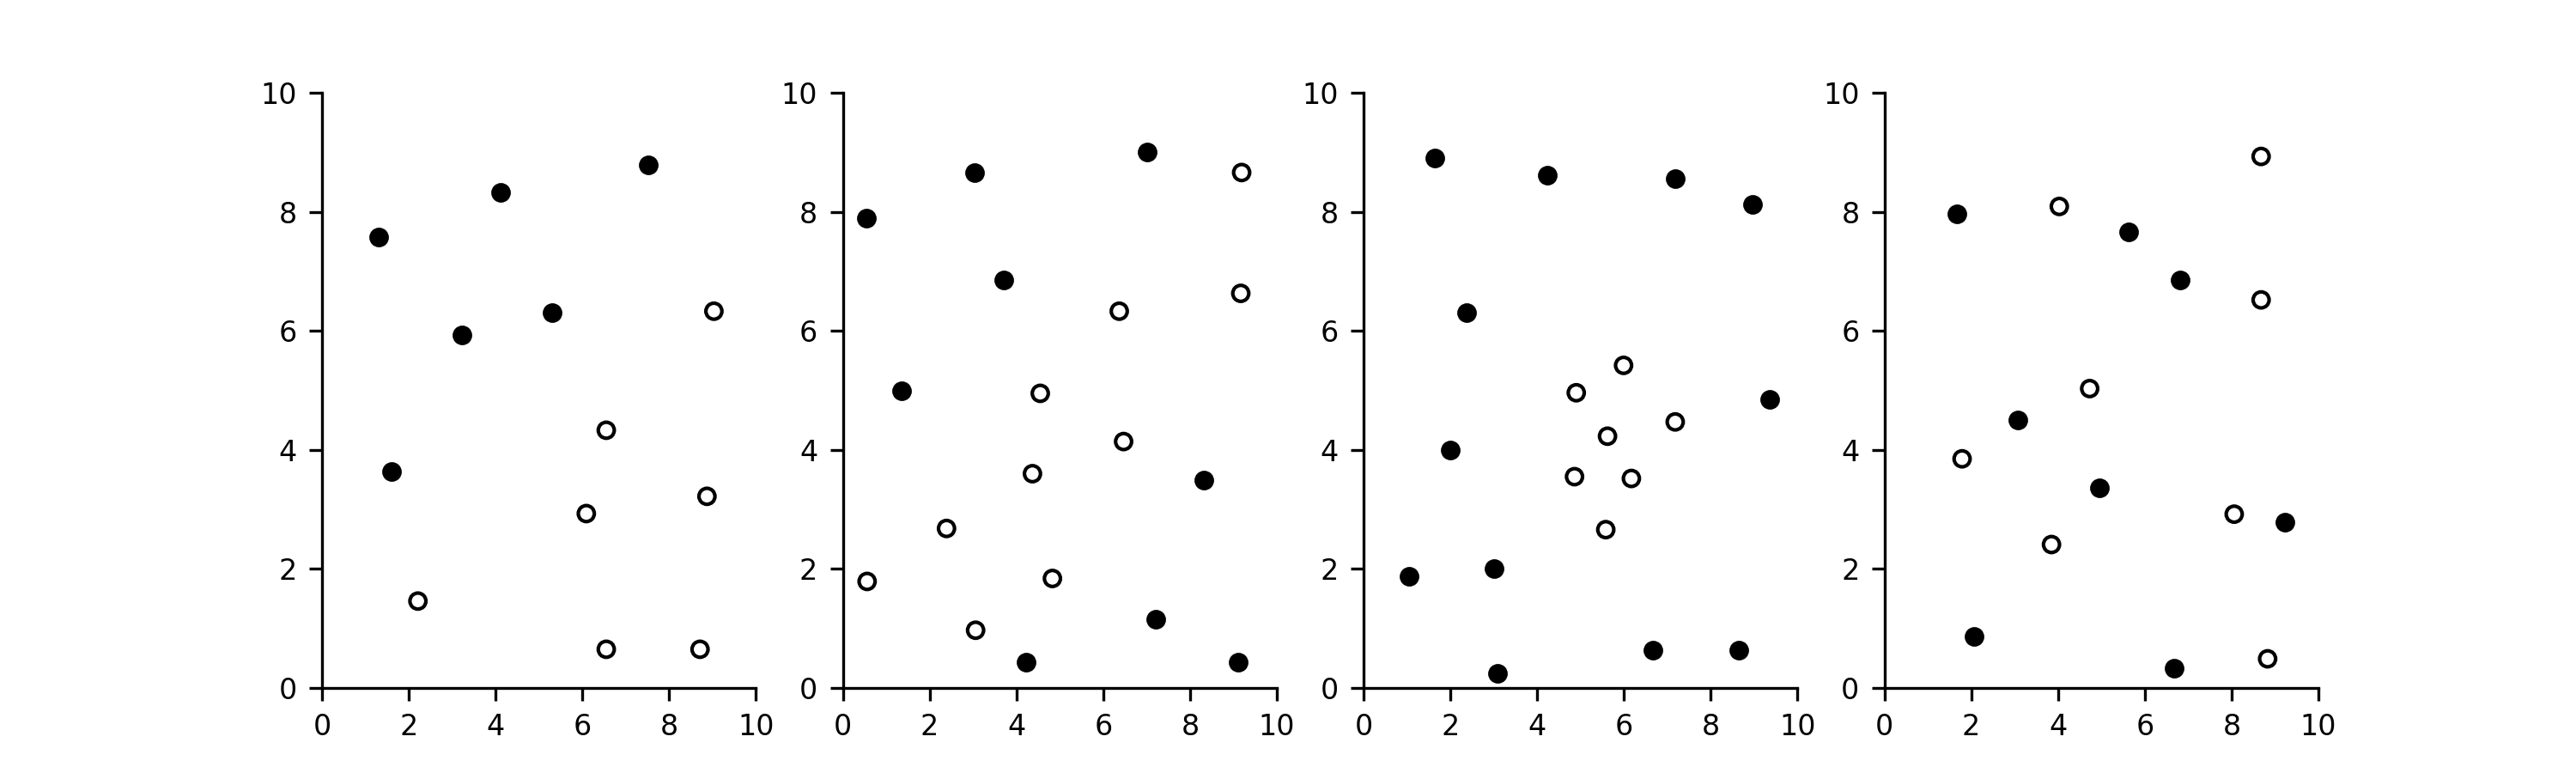
\includegraphics[width=1\linewidth]{"../Chap2/Figures/Fig_linearly_sep.png"}
	\caption{Single layer artificial neural networks such as the perceptron can only classify linearly separable data. (a) is linearly separable. (b) is not linearly separable. However, data are contained in an ellipse. The equation of an ellipse is of the form \(a \times x^2+b\times y^2=1\), so if we transform the feature variables into \(X=x^2\) and \(Y=y^2\), the data become linearly separable. (c) is equivalent to a fundamental XOR gate, and is not linearly separable, which was part of the reasons for the first AI winter. It can either be solved by combining several layers of artificial neurons, or by complex kernel tricks which map the data from the original space into a higher dimensional space where they become linearly separable. (d) is possibly not separable at all. AI: Artificial Intelligence. XOR: Exclusive OR.} 
	\label{fig_linearly_sep}
\end{figure}

\begin{figure}[!ht]
	\centering
	\def\svgwidth{1\columnwidth}
	\fontsize{10pt}{10pt}\selectfont
	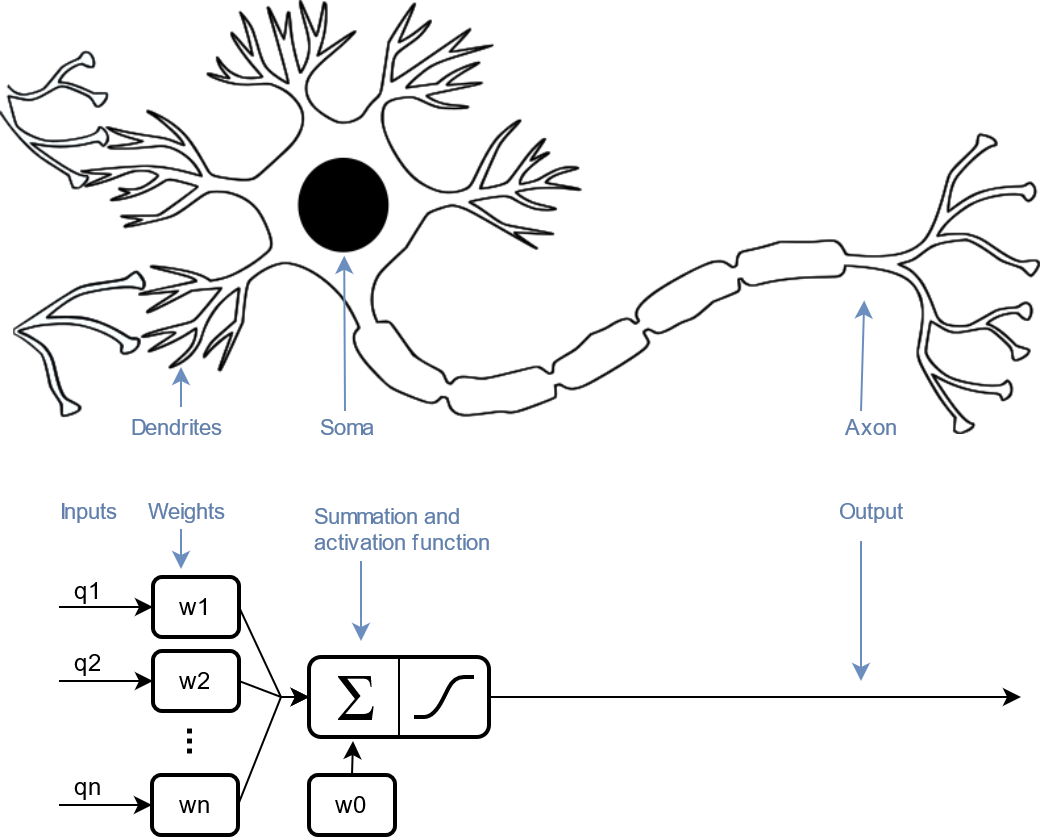
\includegraphics[width=0.95\linewidth]{"../Chap2/Figures/Fig_neuron.png"}
	\caption{The artificial neuron (b) has been modeled after the natural neuron (a). Inputs and weights act as the total nervous influx firing the dendrites. The collected values are summed, and a signal is activated if a threshold is overcome, as the soma does in a natural neuron. The output signal is conveyed the axon in a natural neuron. (b) In the case of a perceptron, the neuron adjusts its weights to minimize the error between the predicted and the expected output. It can be used as a classifier, which outputs class 1 or class 0 depending on the inputs. (c) A dense (fully connected) neural network with one intermediate layer and backpropagation can solve any non-linearly separable classification.}
	\label{fig_neuron}
\end{figure}

\clearpage
\begin{algorithm}[!ht]
  \caption{Perceptron}\label{alg:perceptron}
  \begin{algorithmic}[1]
    \STATEx Let \( \overrightarrow{X^0} \) be the input vector of a first instance of variables \( (1, x_1^0, \cdots x_M^0) \), \( \overrightarrow{W^0} \) the corresponding weights randomly initialized \( (w_0^0, w_1^0, \cdots w_M^0) \) with \(w_0^0\) a bias, and \(y^{0, pred}\) the output predicted binary class. 
    \STATE The summation function is computed: 
    \begin{equation}
        \overrightarrow{W^0} \cdot \overrightarrow{X^0} = \sum_{m \in [0,M]} w_m^0 x_m^0
    \end{equation}
    \STATE This result is processed by an activation function, which is a threshold in the case of the perceptron. It determines whether the neuron will be fired or not, i.e., whether one or the other class will be predicted. $y^{0,pred}$ = 1 corresponds to one class, and $y^{0,pred}$ = 0 to the other. 
    \begin{equation}
        y^{0,pred} = 
        \begin{cases}
            1 & \text{if} \ \overrightarrow{W^0} \cdot \overrightarrow{X^0} > \theta,\\
            0 & \text{otherwise}
        \end{cases}
    \end{equation}
    \STATE This prediction $y^{0,pred}$ is compared to the actual class $y^{0,expected}$. 
    \begin{equation}
        \epsilon^0 = y^{0,expected} - y^{0,pred}
    \end{equation}
    \STATE Then weights are updated: 
    \begin{equation}
        \overrightarrow{W^1} = \overrightarrow{W^0} + \eta \ \epsilon^0 \ \overrightarrow{X^0}
    \end{equation}
    \STATEx with $\eta$ the learning rate $\in$ [0,1]. Note that if the class is correctly predicted, then $\epsilon^0=0$ and weights are not adjusted.   
  %   \STATEx \textit{In Adaline, weights are adjusted early and in a continuous way, before being processed by the activation function: \(\epsilon^0 = \frac{\partial \frac{1}{2}(y^{0,expected} - \overrightarrow{W^0} \cdot \overrightarrow{X^0})^2}{\partial \overrightarrow{W^0}}= y^{0,expected} - \overrightarrow{W^0} \cdot \overrightarrow{X^0}\)}.
  \STATE The algorithm is repeated with another example $\overrightarrow{X^1}$, and so on until it has gone through the whole batch of the training set. If weights still need to be updated, one can go over it again, for a determined number of epochs or until the average error is under a given value. Then the perceptron is considered trained, and ready to correctly predict a class $y$ with the retained weights.
  %   \algstore{alg1}
  \end{algorithmic}
\end{algorithm}

% \begin{algorithm}
%       \begin{algorithmic}[1]
%         \algrestore{alg1}
%         \STATE bla
%       \end{algorithmic}
% \end{algorithm}

\begin{tcolorbox}[nofloat, colback=white,colframe=black, colbacktitle=white, coltitle=black, breakable, title=\textbf{Example 1} Athlete classification with a perceptron, label=example1]
      \phantomsection\hypertarget{example1}
      N.B. The code for running this example is available on the thesis repository \url{https://github.com/davidpagnon/These_David_Pagnon/blob/main/Thesis/Chap2/perceptron.py}.
      \tcblower
      Let's consider force-velocity test results as an input
      \setlength{\belowdisplayskip}{0pt} \setlength{\belowdisplayshortskip}{0pt}
      \setlength{\abovedisplayskip}{0pt} \setlength{\abovedisplayshortskip}{0pt}
      \begin{flalign*}
      \overrightarrow{X} = (1, velocity \ (m/s), force \ (hN) ), && 
      \end{flalign*}
      and the classification of an athlete as "good" or "bad" as an output
      \(y = 1 \ or \ 0. \)\newline
      A batch of training data, i.e., example data the perceptron will learn from, could be: 
      \[ \bigl\{(\overrightarrow{X^i}, y^{i, expected})\bigr\}_{i\in [0,4]}
      = \bigl\{\bigl((1, 1, 5), 1\bigr),
      \bigl((1, 2, 3), 0\bigr),
      \bigl((1, 7, 1), 1\bigr),
      \bigl((1, 4, 1), 0\bigr),
      \bigl((1, 5, 4), 1\bigr)\bigr\}. \]
      
      Let's randomly initialize weights at \(\overrightarrow{W^0} =  (-9, 1, 3) \), take a threshold $\theta$=0.1, and a learning rate $\eta$ = 0.3.\newline
            
      \textbf{The first instance} of the training set gives: 
      \begin{flalign*}
      \overrightarrow{W^0} \cdot \overrightarrow{X^0} = \sum\nolimits_{m \in [0,2]} w_m^0 x^0_m = -9 \times 1+ 1 \times 1 + 3 \times 5 =7.&&
      \end{flalign*}
      Now \(\overrightarrow{W^0} \cdot \overrightarrow{X^0} = 7 > \theta = 0.1\), so $y^{0, pred} = 1$.\newline
      \(y^{0, expected} = 1 = y^{0, pred} \), so the prediction is true and weights don't need to be updated. \newline
      As a consequence, \(\overrightarrow{W^1} = \overrightarrow{W^0} = (-9, 1, 3).\)\newline
      
      \textbf{The second instance} gives \(\overrightarrow{W^1} \cdot \overrightarrow{X^1} = (-9, 1, 3) \cdot (1,2,3) = 2 > \theta = 0.1\), so $y^{1, pred} = 1$. \newline
      But \(y^{1, expected} = 0 \neq y^{1, pred} = 1\), so weights need to be updated.\newline
      The error is \(\epsilon^1 = y^{1,expected} - y^{1,pred} = 0-1 = -1\).\newline
      As a consequence, \(\overrightarrow{W^2} = \overrightarrow{W^1} + \eta \ \epsilon^1 \ \overrightarrow{X^1} = (-9, 1, 3)  + 0.1 \times (-1) \times (1,2,3) = (-9.3,0.4,2.1).\)\newline
      
      \textbf{Third instance}: \(\overrightarrow{W^2} \cdot \overrightarrow{X^2} = (-9.3,0.4,2.1) \cdot (1,7,1) = 3-4.4 < 0.1\), so $y^{2, pred} = 0$. \newline
      \(y^{2, expected} = 1 \neq y^{2, pred} = 0\), so weights need to be updated.\newline 
      \(\epsilon^2 = y^{2,expected} - y^{2,pred} = 1\).\newline
      \(\overrightarrow{W^3} = \overrightarrow{W^2} + \eta \ \epsilon^2 \ \overrightarrow{X^2} = (-9.3,0.4,2.1) + 0.1 \times 1 \times (1,7,1) = (-9,2.5,2.4).\)\newline
      
      \textbf{Fourth instance}: \(\overrightarrow{W^3} \cdot \overrightarrow{X^3} = (-9,2.5,2.4) \cdot (1,4,1) = 3.4 > 0.1\), so $y^{3, pred} = 1$. \newline
      \(y^{3, expected} = 0 \neq y^{3, pred} = 1\), so weights need to be updated.\newline
      \(\epsilon^3 = y^{3,expected} - y^{3,pred} = -1\).\newline
      \(\overrightarrow{W^4} = \overrightarrow{W^3} + \eta \ \epsilon^3 \ \overrightarrow{X^3} = (-9,2.5,2.4) + 0.1 \times (-1) \times (1,4,1) = (-9.3,1.3,2.1).\)\newline
      
      \textbf{Fifth instance}: \(\overrightarrow{W^4} \cdot \overrightarrow{X^4} = (-9.3,1.3,2.1) \cdot (1, 5, 4) = 17.6 > 8\), so $y^{4, pred} = 1$. \newline
      \(y^{4, expected} = 1 = y^{4, pred} = 1\), so weights don't need to be updated.\newline
      \(\overrightarrow{W^5} = \overrightarrow{W^4} = (-9.3,1.3,2.1) (Figure~\ref{fig_perceptron}). \)\newline

      \textbf{Next instances}: Once we have gone over the batch of training data, if the average error is below a given value, we can assume that the perceptron is trained. If not, we can use the next batch to pursue training. If it still didn't converge after all batches, we can iterate over all training data again, for a given number of times. If results are still not satisfying, either the data are not linearly separable, or the training sample is not large enough or of good enough quality. In our case, it seems like our example data have allowed us to correctly separate good and bad athletes based on their force and velocity test results (Figure~\ref{fig_perceptron}).

      {
      \begin{center}
      \def\svgwidth{1\columnwidth}
      \fontsize{10pt}{10pt}\selectfont
      \centerline{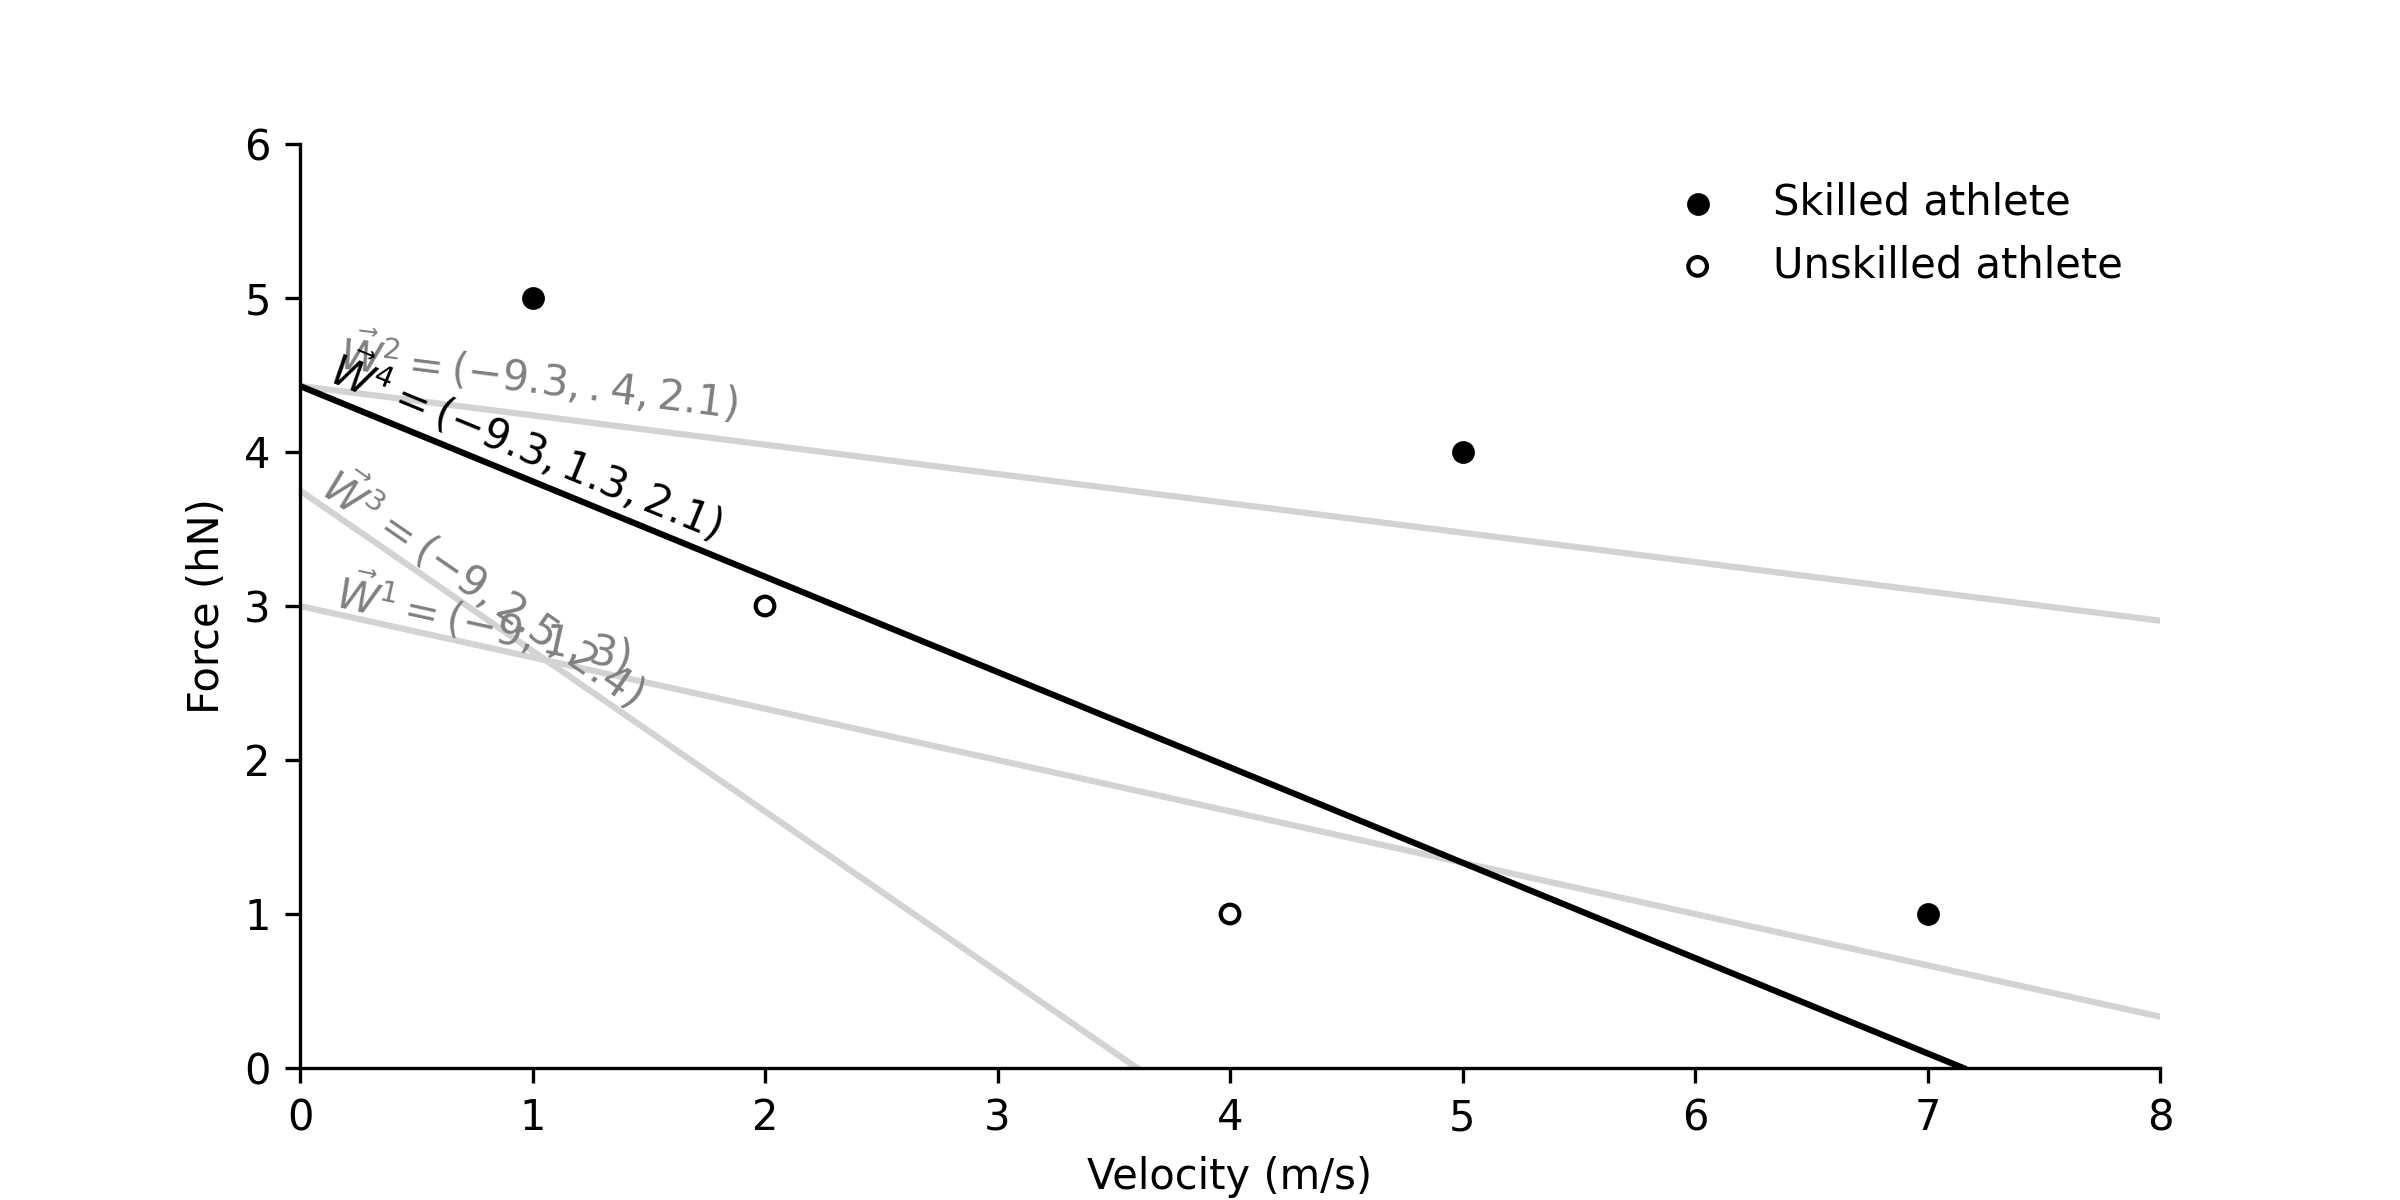
\includegraphics[width=0.9\linewidth]{"../Chap2/Figures/Fig_perceptron.png"}}
      \captionof{figure}{Classification of athletes as "good" (black dot) or "bad" (circle) according to their Force-Velocity results. Weights are adjusted (grey lines), until the perceptron classifies athletes correctly (black line.)}
      \label{fig_perceptron}
      \end{center}
      }
\end{tcolorbox}

\newpage

From the end of the 1990s, there has been no theoretical breakthrough in AI, but larger databases have become available with the advent of the Internet, and greater computational power has become accessible, especially thanks to groundbreaking progress in Graphics Processing Units (GPUs), which made heavy parallel computing available to the wider audience. As a consequence, more layers could be used in neural networks, which progressively set off the onset of deep learning. Finally, complex "common-sense" problems, such as natural language processing or image recognition, could be treated with some success \cite{Baral2018}.

One particular type of deep learning algorithms is the convolutional neural network (CNN), which is particularly suited for image recognition. It was first used for classifying handwritten and low-resolution digits \cite{LeCun1998}, and then applied to more complex images as greater computing resources became available \cite{Krizhevsky2017}. Nowadays, CNNs have sometimes surpassed humans at image classification \cite{Cireşan2012, Lu2015}. A convolution layer consists in a series of filters that slide across the image, each of them outputting a result close to 0 or to 1, depending on how well it can be overlaid on each image area. In the same way as with a simple artificial neuron, each of these filters can be seen as a weight vector \(\overrightarrow{W}\), and each image area as an input vector \(\overrightarrow{X}\). The filters of the first convolution layer are simple patterns such as lines, but then they become circles and corners, until the last layers, when they have developed into complex features corresponding to whole object parts. Once a filter has covered the whole image, it forms a feature map, which will then be downsampled by a pooling layer in order to save computing resources. All the feature maps produced by each filter are processed by a determined number of other convolution layers, and then flattened into a 1D vector. This 1D vector is processed by a few dense layers (dense layers are fully connected, i.e., all outputs are produced by a weighted sum of each input), and lastly a softmax layer computes a probability for the image to correspond to each available class. If the CNN is correctly trained, the class with highest probability corresponds to the correct one: for example, if the image displays a BMX start, the probability for the bike class will be the highest (Figure~\ref{fig_cnn}). 

However, results will not be good until a lot of iterations are done on a lot of data. Indeed, filters at each layer are randomly initialized, and then refined with backpropagation in order to predict all classes as best as possible. One of the risks is overfitting, i.e., to excessively adapt to the training data and to fail to generalize to new data. This is dealt with by cross-validation, i.e., the separation between training and test data, by regularization methods such as radomization, batch normalization and dropout, and by data augmentation, e.g., image rotations, crops, color distortion, noise addition, etc. \cite{Hawkins2004,Chicco2017} (Figure~\ref{fig_xkcd}). An enormous amount of data is also needed to correctly train the CNN, which makes it complicated when unusual classes need to be recognized (for example, a climbing hold, a BMX starting gate, a medial malleolus on the ankle, etc.) Fortunately, one can consider that a CNN trained on a massive dataset, such as ImageNet and its 14 million annotated images \cite{Deng2009}, has learned to recognize most features that can be found in any image. One can take the learned filters of its convolutional layers as is, use them as a feature extractor (sometimes called backbone), and just fine-tune the last dense layers to recognize new classes. It will be much less computationally expensive to train, and will need much fewer data: about a hundred images, instead of thousands. This is called transfer learning \cite{Pan2009}.

Now, classification of a whole image is not sufficient in sports motion analysis. One needs to detect where an object or a person is, and ideally to localize more precise features such as joint centers so as to estimate the person's pose. 

\clearpage
\begin{figure}[hbtp]
	\centering
	\def\svgwidth{1\columnwidth}
	\fontsize{10pt}{10pt}\selectfont
	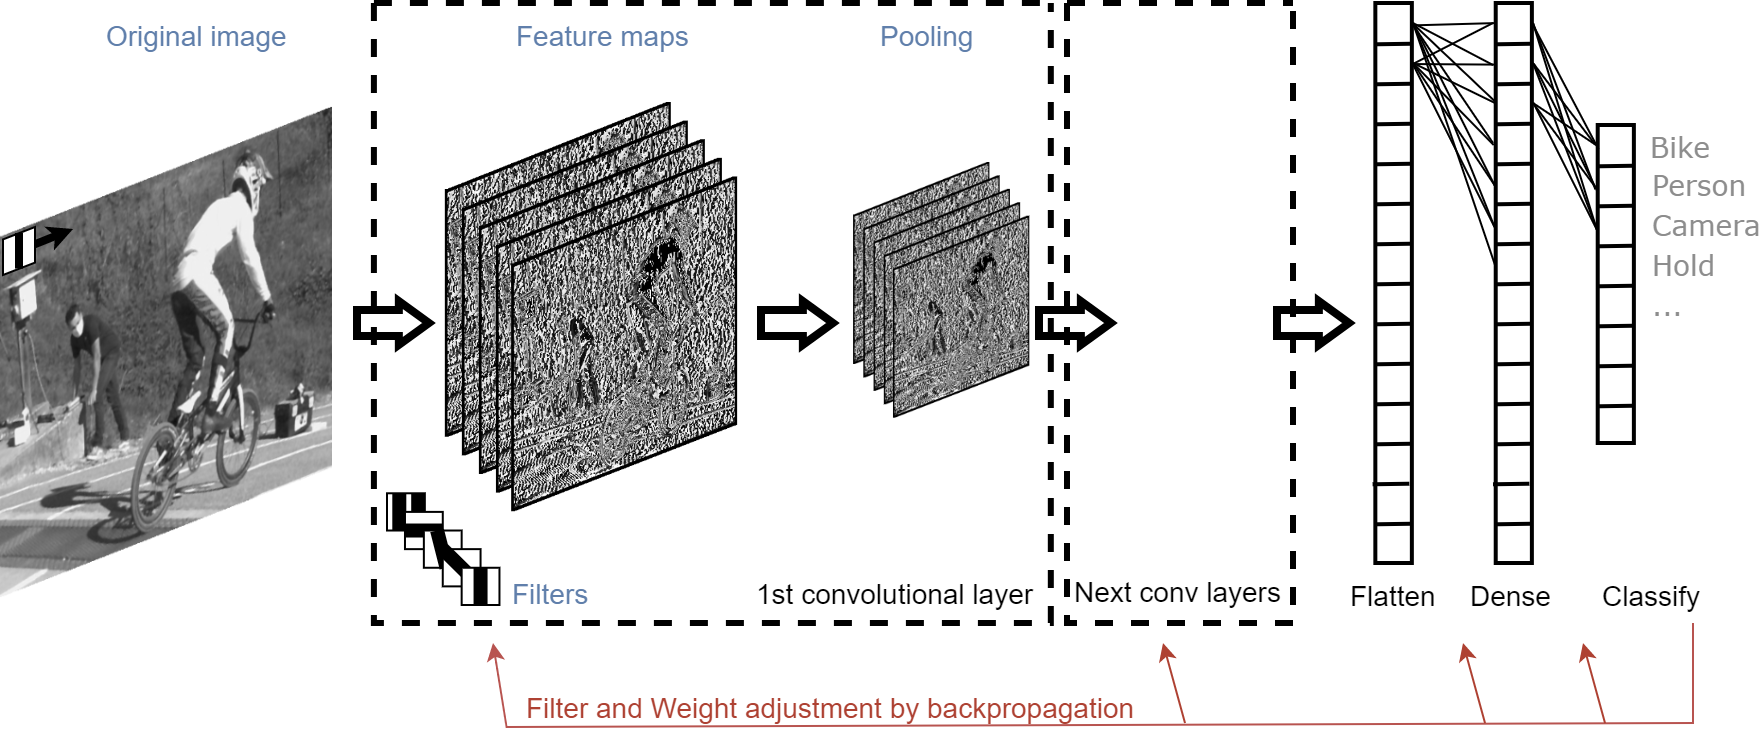
\includegraphics[width=1\linewidth]{"../Chap2/Figures/Fig_CNN.png"}
	\caption{A simplified convolutional neural network (CNN.) A convolutional layer consists in a series of filters running across the input image, and producing feature maps, which are then downsampled by pooling. Filters become more and more elaborated along layers, and produce feature maps which look like whole object parts. Filters and weights are randomly initialized at first, and then are adjusted by backpropagation. After the convolutional layers, the feature maps are flattened to produce a 1D vector, which is then processed by dense layers, and finally a softmax layer computes a probability for the image to correspond to each available class.} 
	\label{fig_cnn}
\end{figure}

\begin{figure}[hbtp]
	\centering
	\def\svgwidth{1\columnwidth}
	\fontsize{10pt}{10pt}\selectfont
	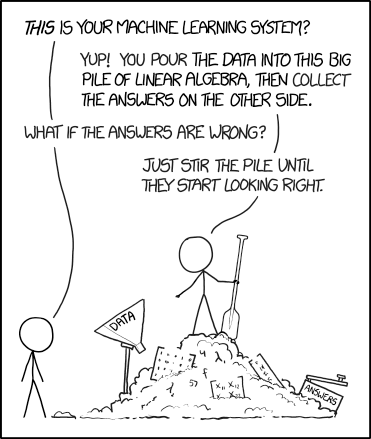
\includegraphics[width=0.4\linewidth]{"../Chap2/Figures/Fig_XKCD.png"}
	\caption{The amazingly rigourous world of machine learning \href{https://xkcd.com/1838/}{XKCD} .} 
	\label{fig_xkcd}
\end{figure}


\subsection{Machine learning for 2D pose detection}\label{sec:Machine learning for 2D pose detection}

Older methods for object detection used to run a sliding and pyramidal window across the image, and then to apply a non-neural classifier on each window, such as an SVM on carefully handcrafted histogram of oriented gradients descriptors (HOG) \cite{Dalal2005}. They then had to be followed by non-maximum suppression, in order to select one bounding box over many overlapping ones. As the classifier is run on each window iteration like if they were independent images, these methods were very computationally intensive, and in the same time not very robust nor accurate. 

\clearpage
More modern approaches are based on CNNs, and as such, they involve a preliminary step: extracting the last layer of a pre-trained neural network such as ImageNet, in order to make it able to classify the objects of interest. One of the precursors, R-CNN (Regions with CNN features) \cite{Girshick2014}, first looks for a lesser amount of regions of interest (ROIs) by selective search, instead of with a sliding window. Selective search is an algorithm which segments image based on pixel intensities, without any learning involved \cite{Uijlings2013}. Then three learning models are used: one CNN for extracting features from each ROI, an SVM for classifying each ROI, and a regression model for adjusting bounding boxes. It takes about 45 seconds to process a single image on benchmarks. Fast R-CNN \cite{Girshick2015} uses one single network for all steps, and switches the first two: it first extracts features from the whole image, and only then uses selective search to find ROIs on the resulting feature map, and finally classifies the ROIs and tightens the bounding boxes. It is much faster and takes about 2 seconds per image. A last incrementation on this basis is Faster R-CNN \cite{Ren2015}, which works similarly to the latter, but finds ROIs with a neural network instead of with selective search, which is very time-consuming. This allows for predicting an "objectness" score on each ROI, and for fitting the bounding boxes directly, and thus on avoiding the last regression step. It is even faster, and takes about 0.2 seconds per image. YOLO (standing for You Only Look Once) \cite{Redmon2016} proposes another approach, and does not separate the steps of finding ROIs with classification. It divides the image into regions, and predicts both classes and bounding boxes for each region. For example, if there is a shoulder in a region, it will predict a "person" class, and a larger box in which this person is likely to fit. YOLO takes about 0.02 seconds per image (45 fps), and is thus able to run real time. However, it is not as accurate as the previous methods, especially on smaller objects. This being said, new versions are very frequently released (although not by the same authors), and the current YOLOv7 \cite{Wang2022b} is both faster and more accurate than all previous approaches as it entirely reviews the whole network architecture to deal with all observed bottlenecks.

But again, in order to perform joint kinematics, one cannot just detect whole objects: precise keypoints need to be localized. Mask R-CNN \cite{He2017}, and the more recent Detectron2 \cite{Wu2019}, still predict the bounding boxes and their class like Faster R-CNN does, but they also add a small overhead in parallel, which predicts the shapes of masks overlaying the object in a pixel-to-pixel manner. Keypoints can be seen as a very small mask, and Mask R-CNN can also detect them in order to predict human pose estimation. In the next paragraph, only multi-person pose estimation models will be considered. Datasets, evaluation metrics, and comparison of results won't be detailed: see \cite{Topham2021} for a comprehensive overview.

Two main approaches for multi-person 2D pose estimation coexist. The "top-down" one first detects bounding boxes around persons, and then finds keypoints inside each box. In the area of object detection methods, they are analogous to region-proposed methods such as the R-CNN suite, which propose ROIs and then find and classify objects. Conversely, the "bottom-up" approach first finds keypoints, and then groups them into persons. They are analogous to the single-shot object detection methods such as the YOLO suite, which first find small details, and then predict full-size objects. These approaches are nowadays almost as fast as the top-down ones, however their inference time does not increase with the amount of persons detected. 

Mask R-CNN belongs to the first kind, as well as AlphaPose \cite{Fang2017}, which mostly differentiates from the latter by using a network predicting higher quality bounding boxes from inaccurate ones, in order to facilitate the task of the joint regressor. On the opposite, DeepCut and DeeperCut \cite{Pishchulin2016,Insafutdinov2016}, as well as DeepLabCut \cite{Mathis2018,Lauer2022} upon which it is built, are bottom-up approaches. They find a large number of keypoint candidates, label them as hand, head, etc., and then select the best candidates and separate them into persons. Since they calculate every possible association between keypoints, this is very slow. OpenPose \cite{Cao2019} uses a network which jointly predicts keypoint locations, and the connections between them (i.e., it also predicts limbs, which define a skeleton), and is much faster while still being accurate. OpenPifPaf \cite{Kreiss2021} adds to it both temporal consistency across frames, and an intensity map for each keypoint instead of punctual locations (i.e., a further keypoint will have a lower intensity). This allows for better accuracy in low-resolution regime and in occluded images. YOLOv7 supports keypoint detection by integrating YOLO-Pose \cite{Maji2022}, and claims to be faster and more accurate than all other state-of-the-art methods. It brings together top-down and bottom-up approaches, and uses a single network predicting both bounding boxes and their corresponding poses. SLEAP \cite{Pereira2022}, which is built for training animal pose estimation models, implements both top-down and bottom-up approaches. In this context, top-down approaches are slightly more accurate, and considerably faster as long as few animals are in the scene.

\begin{figure}[hbtp]
	\centering
	\def\svgwidth{1\columnwidth}
	\fontsize{10pt}{10pt}\selectfont
	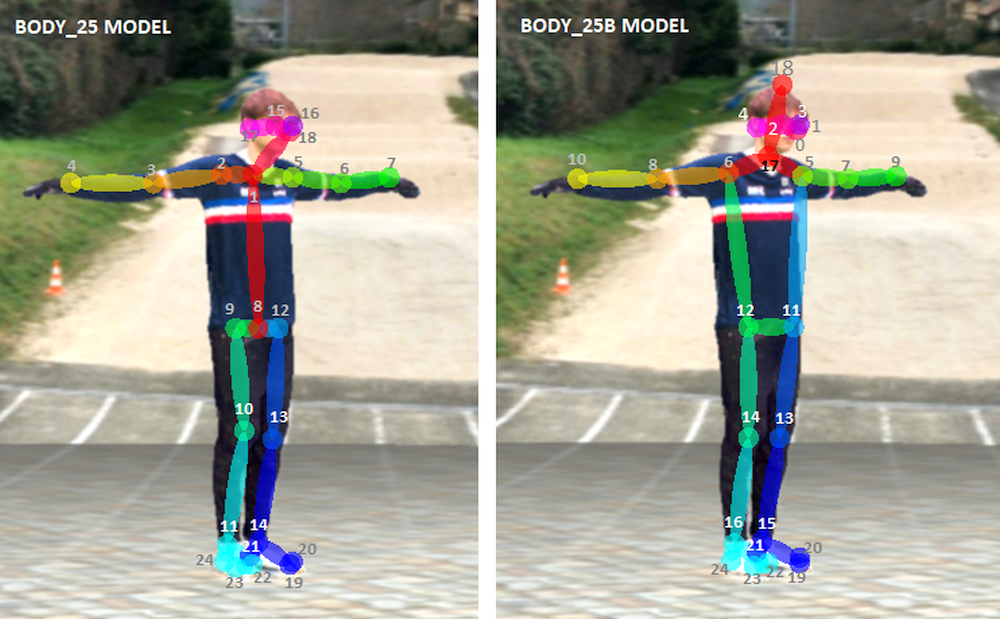
\includegraphics[width=1\linewidth]{"../Chap2/Figures/Fig_body25b.png"}
	\caption{The body\_25b OpenPose model is more accurate than the default body\_25 one. As an example, the left knee is slightly misplaced on the default model. Keypoint definition and order also differ between both models.} 
	\label{fig_body25b}
\end{figure}

Like all previously presented methods, OpenPose has been trained on the COCO dataset \cite{Lin2014}. However, OpenPose body\_25 standard model provides foot keypoints, which are primordial in sports motion analysis. To do so, 6 more keypoints have been labeled for the feet on the COCO dataset before training. OpenPose also supports the single-network whole-body pose estimation network \cite{Hidalgo2019}, which has been trained in the same time on COCO+foot,  MPII \cite{Andriluka2014}, and on Total Capture \cite{Xiang2019} in order to provide hand, face, feet, and body keypoints in one single network. A submodel of it is body\_25b, which provides body and foot keypoints as body\_25 does (although in slightly different locations), and in addition decreases the number of false positives without hampering speed (Figure~\ref{fig_body25b}). In a similar way, AlphaPose provides full-body models, either trained on the Halpe dataset \cite{Li2020}, or on the COCO-WholeBody one \cite{Xu2022}. Note that BlazePose \cite{Bazarevsky2020}, trained on the GHUM dataset \cite{Xu2020b}, also provides hand and feet keypoints, but since it is a single-person pose estimation model, the architecture is different and will not be addressed here. Indeed, this is rarely suitable in sports conditions, where people are usually present in the background. 


\FloatBarrier
\section{3D reconstruction}\label{sec:3D reconstruction}
\label{ch:2.2}

Once the pose of an athlete is correctly detected, the next step is to obtain their 3D pose. While some approaches strive to infer 3D pose from a monocular video source, they are generally not considered sufficiently accurate, especially when body parts are occluded. It is, then, important to use several cameras, and to fuse their 2D pose estimation results to obtain more reliable 3D coordinates.


\subsection{Pinhole camera model}\label{subsec:Pinhole model}

camera coordinate system


% https://ressources.unisciel.fr/DAEU/physique/bases-optique/co/Lent_Conjugaison.html
% http://www.optique-ingenieur.org/fr/cours/OPI_fr_M04_C01/co/Contenu01.html
% https://en.wikipedia.org/wiki/Camera
% https://en.wikipedia.org/wiki/Camera_obscura
% https://en.wikipedia.org/wiki/Pinhole_camera
% https://fr.wikipedia.org/wiki/Calibration_de_cam%C3%A9ra
% https://docs.opencv.org/4.x/d9/db7/tutorial_py_table_of_contents_calib3d.html
% https://docs.opencv.org/4.x/d6/d55/tutorial_table_of_content_calib3d.html




\subsection{Calibration}

\cite{Marchand2015}


\subsection{Triangulation}\label{triangulation}

Algorithm~\ref{alg:dlt} for a proof of the classic direct linear transform (DLT), commonly used to solve the triangulation of 2D coordinates from several cameras with a least square approach.


\begin{algorithm}[!ht]
      \caption{Direct Linear Transform (DLT)}\label{alg:dlt}
      \begin{algorithmic}[1]
          \STATEx Let \(\overrightarrow{Q} = (X, Y, Z, 1)\) be the homogeneous coordinates of a 3D object point, 
          \STATEx \(\overrightarrow{q} = (u, v, 1)\) the homogeneous coordinates of a 2D image point on a given camera,
          \STATEx \(\textbf{P} = (P_1^T, P_2^T, P_3^T, P_4^T)\) the projection matrix of the same camera, with \(P_1^T, P_2^T, P_3^T, P_4^T\) the rows of \textbf{P}, and \(\lambda\) an unknown scale factor. 
          \STATE The equation
            \begin{equation}
              \lambda \overrightarrow{q} = \bm{P} \overrightarrow{Q}
            \end{equation}
            may be written as
            \begin{equation}
              \begin{aligned}
              &\lambda u = P_1^T \overrightarrow{Q},\\
              &\lambda v = P_2^T \overrightarrow{Q},\\
              &\lambda = P_3^T \overrightarrow{Q},
              \end{aligned}
            \end{equation}
            which gives two equations:
            \begin{equation}\label{eq:dlt}
              \begin{aligned}
              &(P_1^T - u P_3^T) \overrightarrow{Q} = 0,\\
              &(P_2^T - v P_3^T) \overrightarrow{Q} = 0
              \end{aligned}
            \end{equation}
      \STATE With N cameras, we obtain a system of 2N equations that can be written in the form:
      \begin{equation}
        \textbf{A} \overrightarrow{Q} = 0.
      \end{equation}
      \STATE A singular value decomposition (SVD) of \textbf{A} gives 
      \begin{equation}
        A = \textbf{U} \textbf{S} \textbf{V}^T
      \end{equation}
      with \(\textbf{U}, \textbf{V}\) orthonormal basis, and \(\textbf{S}\) the diagonal matrix filled with the singular values of \textbf{A}, namely \(\sigma_1, \sigma_2, \sigma_3, \sigma_4\). \(\overrightarrow{Q}\) can be expressed as 
      \begin{equation}
        \overrightarrow{Q} = \textbf{V} \overrightarrow{\alpha},
      \end{equation}
      with \(\overrightarrow{\alpha} = \begin{pmatrix}\alpha_1 \\\alpha_2 \\\alpha_3 \\\alpha_4\end{pmatrix}\). The Python function \href{https://numpy.org/doc/stable/reference/generated/numpy.linalg.svd.html}{numpy.linalg.svd()} can swiftly compute SVDs. 
      \algstore{alg1}
    \end{algorithmic}
\end{algorithm}

\begin{algorithm}
      \begin{algorithmic}[1]
        \algrestore{alg1}
      \STATE Unless all projection matrices and all image points are perfectly determined, \(\textbf{A}\overrightarrow{Q} \neq 0\). However, it is possible to find a least square solution for our 3D object point \(\overrightarrow{Q}\). Indeed, minimizing \((\textbf{A}\overrightarrow{Q})^2\) also minimizes \(\textbf{A}\overrightarrow{Q}\).
      \begin{equation}
          \begin{aligned}
          (\textbf{A}\overrightarrow{Q})^2 & = (\textbf{A} \overrightarrow{Q})^T (\textbf{A} \overrightarrow{Q})\\
          & = (\overrightarrow{\alpha}^T \textbf{V}^T \ \textbf{V} \textbf{S} \textbf{U}^T)(\textbf{U} \textbf{S} \textbf{V}^T \ \textbf{V}\overrightarrow{\alpha})\\
          & = \overrightarrow{\alpha}^T \textbf{S} \overrightarrow{\alpha}\\
          & = \sum_{i \in [1,4]} \alpha_i^2 \sigma_i^2
          \end{aligned}
      \end{equation}
      which is minimum when all \(\alpha\) factors are set to zero, except the factor of the smallest singular value \(\sigma\). 
      \STATE Assuming that \(\sigma_{min} = \sigma_4\), then \((\textbf{A}\overrightarrow{Q})^2\) is minimum when \(\alpha_1, \alpha_2, \alpha_3\) are null.
      \begin{equation}
          (\textbf{A} \overrightarrow{Q})_{min} = \alpha_4 \sigma_4
      \end{equation}
      and 
      \begin{equation}
          \overrightarrow{Q} = 
          \textbf{V} \overrightarrow{\alpha} 
          = \begin{pmatrix}V_{11} & V_{12} & V_{13} & V_{14} \\
          V_{21} & V_{22} & V_{23} & V_{24} \\
          V_{31} & V_{32} & V_{33} & V_{13} \\
          V_{41} & V_{42} & V_{43} & V_{44}\end{pmatrix} \begin{pmatrix}0 \\0 \\0 \\\alpha_4\end{pmatrix} 
          = \alpha_4 \begin{pmatrix}V_{14} \\V_{24} \\V_{34} \\V_{44}\end{pmatrix} 
          = \begin{pmatrix}X \\Y \\Z \\1\end{pmatrix}
      \end{equation} 
      \STATE As a consequence, the triangulated point is equal to
      \begin{equation}
          \overrightarrow{Q}=\begin{pmatrix}X \\Y \\Z \\1\end{pmatrix} = \begin{pmatrix}V_{14}/V_{44} \\V_{24}/V_{44} \\V_{34}/V_{44} \\1\end{pmatrix}
      \end{equation}
      \end{algorithmic}
\end{algorithm}




\section{3D joint kinematics}\label{sec:3D joint kin}


---Direct kinematics
6 DoF 

1 reference frame / coordinate system per segment (at least 3 markers per segment) \cite{Wu2002, Wu2005}
no need for assumptions. Free bodies



---Inverse kinematics 
Model-based

initially for 3D animation applications

Model based:
- model, kinematic chain
- scaling
- IK
IK vs forward kinematics (joint angles -> segment orientation)


Theory: weighted least square/convex/non-linear optimization by OpenSim (vs. Jacobian inverse/Levenberg-Marquardt, vs. heuristic methods)


Global optimization / multibody kinematic optimization, reduces sensitivity to soft tissue artifact, reduces number of degrees of freedom to solve, and thus of markers needed (1 per joint if fully constrained \cite{Slater2018}, vs. 3 min for 6DoF, no need for interpolation or redo capture if marker falls) -> Fohanno2014?, more potential information on muscle activation for example \cite{Robinson2013,Kainz2016}
Slightly slower, assumes that all human beings have similar joint mechanics, based on \textit{a priori} constraints inferred from observations of a population, not garanteed to work on pathological population nor on unusual body structures (joint laxity cannot be qualified for example)

Résultats similaires si STA limités et modèle approprié \cite{Kainz2016}




\subsection{Physically consistent model}

autre


\subsection{Scaling}

bref


\subsection{Inverse kinematics}



As opposed to forward kinematics \newline
Compare with 2D angles between 3 points \newline
Different methods (model based vs autres) for angles (cf mail starred)\newline


Model constrained, based on mechanical joint modeling, and on constraints inferred from  
optimize the posture of a physically consistent skeleton, scaled to each individual subject. In particular, this allows for obtaining 3D joint angles at each point in time, commonly referred to as inverse kinematics (IK.)







%%%%%%%%%%%%%%%%%%%%%%%%%%%%%%%%%%%%%%%%%%%%%%%%%%%%%%%%%%%%
% Intéressant mais rendrait le pdf trop long               %
%%%%%%%%%%%%%%%%%%%%%%%%%%%%%%%%%%%%%%%%%%%%%%%%%%%%%%%%%%%%

% Perceptron (perceptron rule)
% Adaline (delta rule, linear activation function, gradient descent) \cite{Widrow1960}
% Logistic regression (sigmoid activation function, softmax) -> multi-layer
% Neats (basic principles extended to general intelligence) vs scruffies (specific solutions for each problem, cf expert systems)
% SVM (maximizes distance points to line), Random forest
% Linearly separable problems: use of complex "kernel tricks" \cite{Aizerman1964}, popularized by Hofmann in 2008
% supervised vs unsupervised learning
% Issues such as vanishing gradient, overfitting (data augmentation, regularization, dropout, batch normalization)
% feed-forward vs recurrent neural networks
% Classification vs Regression (to get numbers, locations, or parameters, instead of classes), reinforcement learning, adversarial networks, etc.
% Other versions of yolo, ssd
% single person detector such as stacked hourglass, etc
% parametric: adjusts parametes of a model (cf SMPL: silhouette prediction and then 3D shape parameters prediction, and then regression from vertices to 3D joint locations) vs non-parametric: finds keypoinds anywhere in the image (cf OpenPose)
% discriminative vs generative
% Different architectures, different datasets & models
% Attention body_25b: body plus précis (1%: 66.4 vs 65.3 AP), mais foot moins (76.8 vs 77.9 AP. Mais foot plutôt précis dans tous les cas). Egalement: si on applique le réseau aussi au face+hands, on ne gagne rien sur la précision du body (mais plus précis sur face & hand, et bien sûr plus rapide que body+face+hands indépendament). 


% Adaline \cite{Widrow1960} is an improved version of the perceptron, which introduces the concept of gradient descent. It converges faster as weights are adjusted early and in a continuous way, by directly using the result of the summation function instead of processing it with a binary activation function \(\epsilon^0 = \frac{\partial \frac{1}{2}(y^{0,actual} - \overrightarrow{W^0} \cdot \overrightarrow{X^0})^2}{\partial \overrightarrow{W^0}}= y^{0,actual} - \overrightarrow{W^0} \cdot \overrightarrow{X^0}\). As a consequence, the weights are more or less heavily adjusted depending on how large the error is, in an adaptive way (hence its name, which stands for Adaptive Linear Element.) 

% Non-linear problems can either be solved by using multi-layer neural networks with backpropagation, or by using kernel tricks \cite{Aizerman1964}. Kernel tricks consist in mapping the input data into a higher dimensional space, where they become linearly separable. However, although the concepts had been introduced early, they have not been connected to this particular problem until much later.


%%%%%%%%%%%%%%%%%%%%%%%%%%%%%%%%%%%%%%%%%%%%%%%%%%%%%%%%%%%%%%%
% Figure example perceptron                                   %
%%%%%%%%%%%%%%%%%%%%%%%%%%%%%%%%%%%%%%%%%%%%%%%%%%%%%%%%%%%%%%%

% \begin{figure}[hbtp]
% 	\centering
% 	\def\svgwidth{1\columnwidth}
% 	\fontsize{10pt}{10pt}\selectfont
% 	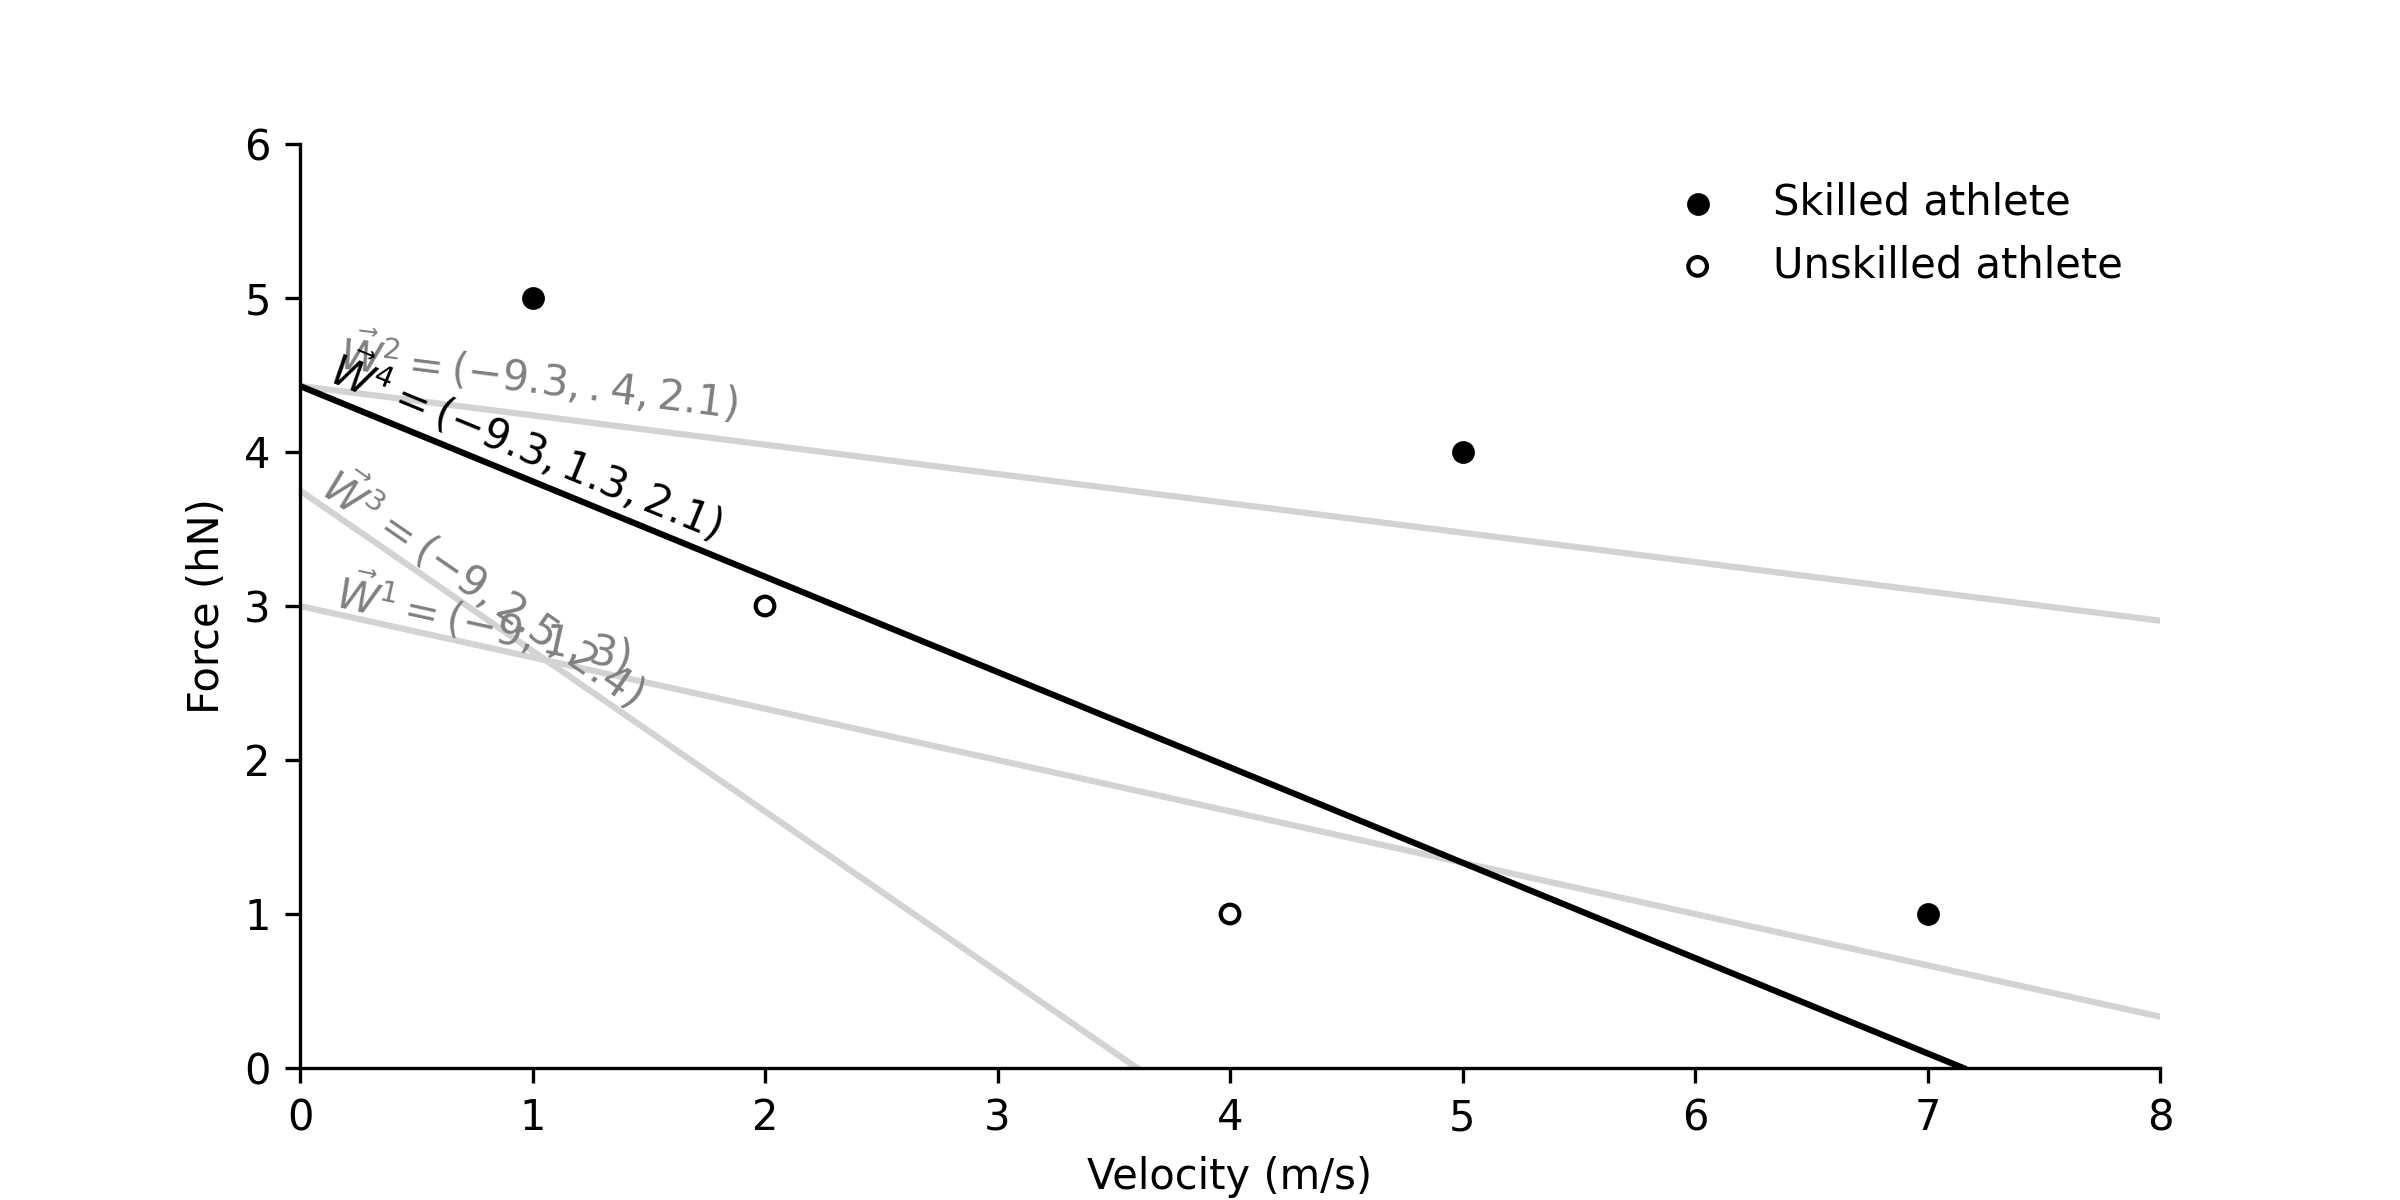
\includegraphics[width=\linewidth]{"../Chap2/Figures/Fig_perceptron.png"}
% 	\caption{Classification of athletes as "good" (black dot) or "bad" (circle) according to their Force-Velocity results. Weights are adjusted (grey lines), until the perceptron classifies athletes correctly (black line.)}
% 	\label{fig_perceptron}
% \end{figure}

% % En tikz
% \begin{figure}
% \centering
% \begin{tikzpicture}[x=0.5cm, y=0.5cm]
%     \draw[thick,->] (0,0) -- (0,6) node[anchor=south east] {Force (hN)};
%     \draw[thick,->] (0,0) -- (10,0) node[anchor=north west] {velocity (m/s)};
%     \foreach \x in {0,1,2,3,4,5,6,7,8,9}
%         \draw (\x,1pt) -- (\x,-1pt) node[anchor=north] {$\x$};
%     \foreach \y in {0,1,2,3,4,5}
%         \draw (1pt,\y) -- (-1pt,\y) node[anchor=east] {$\y$};
%     \foreach \Point in {(1,5), (5,4), (7,1)}{
%       \node at \Point {\textbullet};}
%     \foreach \Point in {(2,3), (4,1)}{
%       \node at \Point {$\circ$};}
%     % \node [green] at (5,4) {\textbullet};
%     % \node [red] at (2,3) {$\circ$};
%     \end{tikzpicture}
% \caption{Force-velocity results and classification.}
% \end{figure}

% % En matplotlib
% # Found on https://stackoverflow.com/questions/19907140/keeps-text-rotated-in-data-coordinate-system-after-resizing
% import matplotlib.pyplot as plt
% import numpy as np
% plt.rcParams.update({'font.size': 10})
% #import matplotlib.mathtext as mathtext
% import matplotlib.text as mtext
% import matplotlib.transforms as mtransforms

% class RotationAwareAnnotation(mtext.Annotation):
%     def __init__(self, s, xy, p, pa=None, ax=None, **kwargs):
%         self.ax = ax or plt.gca()
%         self.p = p
%         self.pa = pa
%         if not pa:
%             self.pa = xy
%         self.calc_angle_data()
%         kwargs.update(rotation_mode=kwargs.get("rotation_mode", "anchor"))
%         mtext.Annotation.__init__(self, s, xy, **kwargs)
%         self.set_transform(mtransforms.IdentityTransform())
%         if 'clip_on' in kwargs:
%             self.set_clip_path(self.ax.patch)
%         self.ax._add_text(self)

%     def calc_angle_data(self):
%         ang = np.arctan2(self.p[1]-self.pa[1], self.p[0]-self.pa[0])
%         self.angle_data = np.rad2deg(ang)

%     def _get_rotation(self):
%         return self.ax.transData.transform_angles(np.array((self.angle_data,)), 
%                             np.array([self.pa[0], self.pa[1]]).reshape((1, 2)))[0]

%     def _set_rotation(self, rotation):
%         pass

%     _rotation = property(_get_rotation, _set_rotation)

% plt.figure(figsize=(8, 4))
% plt.axis([0, 8, 0, 6])
% plt.gca().spines['top'].set_visible(False)
% plt.gca().spines['right'].set_visible(False)
% plt.gca().set_xlabel('Velocity (m/s)')
% plt.gca().set_ylabel('Force (hN)')

% velocity_good = [1,5,7]
% force_good = [5,4,1]
% velocity_bad = [2,4]
% force_bad = [3,1]
% plt.scatter(velocity_good, force_good, s=20, edgecolors='k', facecolors='k', label = "Good athlete")
% plt.scatter(velocity_bad, force_bad, s=20, edgecolors='k', facecolors='none', label="Bad athlete")
% plt.legend(frameon=False)

% # First lines with first weights, with dash greyed lines and label
% W=[-9,  1,  3]
% x1 = np.array( [0, -W[0]/W[1]] )
% x2 = np.array( [-W[0]/W[2], 0] )
% plt.plot(x1,x2, 'lightgrey')
% RotationAwareAnnotation(r'$\vec{W}^1=(-9,1,3)$', 
%       xy=(.15,3.3), p=[-W[0]/W[1],0], pa=[0,-W[0]/W[2]], ax=plt.gca(), xytext=(2,-1), textcoords="offset points", va="top", c='grey', bbox=dict(facecolor='None', edgecolor='None'))
    
% W=[-9.3, .4,  2.1]
% x1 = np.array( [0, -W[0]/W[1]] )
% x2 = np.array( [-W[0]/W[2], 0] )
% plt.plot(x1,x2, 'lightgrey')
% RotationAwareAnnotation(r'$\vec{W}^2=(-9.3, .4,  2.1)$', 
%       xy=(.15,4.85), p=[-W[0]/W[1],0], pa=[0,-W[0]/W[2]], ax=plt.gca(), xytext=(2,-1), textcoords="offset points", va="top", c='grey', bbox=dict(facecolor='None', edgecolor='None'))

% W=[-9,  2.5, 2.4]
% x1 = np.array( [0, -W[0]/W[1]] )
% x2 = np.array( [-W[0]/W[2], 0] )
% plt.plot(x1,x2, 'lightgrey')
% RotationAwareAnnotation(r'$\vec{W}^3=(-9,2.5,2.4)$', 
%     xy=(.15,4), p=[-W[0]/W[1],0], pa=[0,-W[0]/W[2]], ax=plt.gca(), xytext=(2,-1), textcoords="offset points", va="top", c='grey', bbox=dict(facecolor='None', edgecolor='None'))

% W=[-9.3,  1.3, 2.1]
% x1 = np.array( [0, -W[0]/W[1]] )
% x2 = np.array( [-W[0]/W[2], 0] )
% plt.plot(x1,x2, 'k')
% RotationAwareAnnotation(r'$\vec{W}^4=(-9.3,  1.3, 2.1)$', 
%       xy=(.15,4.75), p=[-W[0]/W[1],0], pa=[0,-W[0]/W[2]], ax=plt.gca(), xytext=(2,-1), textcoords="offset points", va="top", bbox=dict(facecolor='None', edgecolor='None'))

% plt.savefig(r'D:\softs\github_david\These_David_Pagnon\Thesis\Chap2\Figures\Fig_perceptron', dpi=300)
% plt.show()


%%%%%%%%%%%%%%%%%%%%%%%%%%%%%%%%%%%%%%%%%%%%%%%%%%%%%%%%%%%%%%%
% Figure linearly separable                                   %
%%%%%%%%%%%%%%%%%%%%%%%%%%%%%%%%%%%%%%%%%%%%%%%%%%%%%%%%%%%%%%%

% import matplotlib.pyplot as plt
% import numpy as np
% plt.rcParams.update({'font.size': 8})

% # Place dots on graph on click and record position
% # adapted from https://stackoverflow.com/a/41825214/12196632
% fig = plt.figure()
% ax = fig.add_subplot(111)
% ax.set_xlim([0, 10])
% ax.set_ylim([0, 10])

% def onclick(event):
%     print(f'{event.xdata}, {event.ydata}')
%     plt.plot(event.xdata, event.ydata, 'o')
%     fig.canvas.draw()
% cid = fig.canvas.mpl_connect('button_press_event', onclick)
% plt.show()


% # Plot examples of linearly and non-liearly separable data
% fig, axs = plt.subplots(1,4,figsize=(10,3))
% plt.rcParams.update({'font.size': 8})

% axs[0].scatter([1.31,4.11,3.22,1.61,5.30,7.52], [7.58,8.33,5.93,3.63,6.31,8.79],s=20, edgecolors='k', facecolors='k')
% axs[0].scatter([6.55,8.71,8.87,9.03,6.55,2.21,6.09], [0.65,0.65,3.22,6.33,4.33,1.46,2.93],s=20, edgecolors='k', facecolors='None')
% axs[0].plot([0,10],[1,10])
% axs[0].text(0.5,0.5,'(a)')

% axs[1].scatter([1.65,4.23,2.38,1.05,3.08,8.65,9.35,8.97,6.67, 7.19,3.00,2.00], [8.91,8.61,6.31,1.87, 0.25,0.63,4.85,8.12,0.63,8.55,2.00,4.00],s=20, edgecolors='k', facecolors='k')
% axs[1].scatter([4.90,4.86,6.17,5.62,5.99,5.58,7.18], [4.96,3.55,3.52,4.23,5.42,2.66,4.47],s=20, edgecolors='k', facecolors='None')
% t = np.linspace(0, 2*np.pi, 100)
% axs[1].plot(6+1.8*np.cos(t) , 4+2*np.sin(t),'-')
% axs[1].text(0.5,0.5,'(b)')

% axs[2].scatter([0.54,3.04,7.01,3.70,1.35,4.23,7.21,9.11,8.32], [7.90, 8.66,9.01,6.85,5.00,0.44,1.16,0.43,3.49],s=20, edgecolors='k', facecolors='k')
% axs[2].scatter([0.56,2.39,4.55,9.19,6.37,6.47,3.06,4.37,9.17,4.83], [1.79,2.68,4.95,8.66,6.33,4.14,0.97,3.60,6.63,1.84],s=20, edgecolors='k', facecolors='None')
% axs[2].plot([0,10],[2,10])
% axs[2].plot([3,10],[0,5], c='tab:blue')
% axs[2].text(0.5,0.5,'(c)')

% axs[3].scatter([1.67,3.08,6.81,9.23,6.67,2.06,4.96,5.62], [7.96,4.50,6.85,2.79,0.33,0.87,3.36,7.66],s=20, edgecolors='k', facecolors='k')
% axs[3].scatter([8.68,1.79,3.85,4.73,4.03,8.06,8.83,8.68], [6.52,3.85,2.41,5.03,8.09,2.92,0.49,8.93],s=20, edgecolors='k', facecolors='None')
% axs[3].text(5,3.5,'?',fontsize=70, **{'color':'tab:blue', 'fontfamily':'monospace'})
% axs[3].text(0.5,0.5,'(d)')

% for ax in axs:
%     ax.set_xlim([0, 10])
%     ax.set_ylim([0, 10])
%     ax.spines['top'].set_visible(False)
%     ax.spines['right'].set_visible(False)

% fig.savefig(r'D:\softs\github_david\These_David_Pagnon\Thesis\Chap2\Figures\Fig_linearly_sep', dpi=300)
% fig.show()


%%%%%%%%%%%%%%%%%%%%%%%%%%%%%%%%%%%%%%%%%%%%%%%%%%%%%%%%%%%%%%%
% Simple 3x3 line filter on image                             %
%%%%%%%%%%%%%%%%%%%%%%%%%%%%%%%%%%%%%%%%%%%%%%%%%%%%%%%%%%%%%%%

% # # Inspired from https://www.codingame.com/playgrounds/2524/basic-image-manipulation/filtering

% import cv2
% import numpy as np
% import os

% # Load image:
% dir_path = r'D:\softs\github_david\These_David_Pagnon\Thesis\Chap2\Figures'
% input_image = cv2.imread(os.path.join(dir_path,r"out_skewed.png"))
% width, height, _ = input_image.shape

% ## Calculate pixel intensity as the average of red, green and blue colors.
% intensity = [[sum(input_image[x, y]) / 3 for y in range(height)] for x in range(width)]

% # Line filter
% kernelx = [[-1, 0, 1],
%            [-2, 0, 2],
%            [-1, 0, 1]]
% # kernelx = [[-2,-1, 0, 1, 2],
% #            [-2,-1, 0, 1, 2],
% #            [-3,-2, 0, 2, 3],
% #            [-2,-1, 0, 1, 2],
% #            [-2,-1, 0, 1, 2]]

% # Create output image
% output_image = input_image.copy()

% # Compute convolution between intensity and kernels
% for x in range(1, width - 1):
%     for y in range(1, height - 1):
%         magx, magy = 0, 0
%         for a in range(3):
%             for b in range(3):
%                 xn = x + a - 1
%                 yn = y + b - 1
%                 magx += intensity[xn][yn] * kernelx[a][b]

%         # Draw in black and white the magnitude
%         output_image[x, y] = (magx, magx, magx)

% # Transform black pixels to transparent
% # alpha = np.sum(output_image, axis=-1) > 0  
% # alpha = np.uint8(alpha * 255)
% # output_image = np.dstack((output_image, alpha))

% # cv2.imshow('',output_image)
% cv2.imwrite(os.path.join(dir_path,r"out.png"), output_image)